\item \textbf{Augmented Reality for Enhanced Interaction and Safety}
   % Augmented reality user interface design and experimental evaluation for human-robot collaborative assembly - reference : CHU2023313
    % Leveraging \ac{AR} can significantly improve the interaction between humans and robots by providing intuitive visualizations and reducing the need 
    % for continuous visual contact. As demonstrated by Chu et al. \cite{CHU2023313}, effectively conveying robot intentions through \ac{AR} visuals enhances 
    % worker awareness of their surroundings, thereby improving safety and efficiency in collaborative tasks. 
    
    % After analysing previous related work and implemented methodologies, 

    % The \ac{AR} interfaces clearly visualize the 
    % robot's work envelope, as depicted in Figure~\ref{fig:ar-envelope}, enabling human operators to navigate shared workspaces safely and efficiently.
    
    % \begin{figure}[htp]
    %     \centering
    %     \begin{subfigure}{.5\textwidth}
    %         \centering
    %         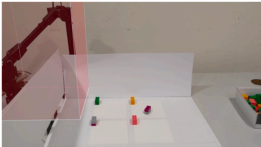
\includegraphics[width=0.9\linewidth]{figs/a-work-env.png}
    %         \caption{}
    %         \label{fig:sfig1}
    %     \end{subfigure}%
    %     \begin{subfigure}{.5\textwidth}
    %         \centering
    %         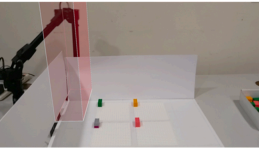
\includegraphics[width=0.9\linewidth]{figs/b-work-env.png}
    %         \caption{}
    %         \label{fig:sfig2}
    %     \end{subfigure}
    %     \begin{subfigure}{.5\textwidth}
    %         \centering
    %         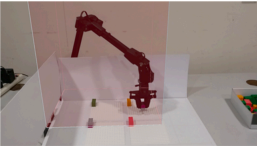
\includegraphics[width=0.9\linewidth]{figs/c-work-env.png}
    %         \caption{}
    %         \label{fig:sfig3}
    %     \end{subfigure}%
    %     \begin{subfigure}{.5\textwidth}
    %         \centering
    %         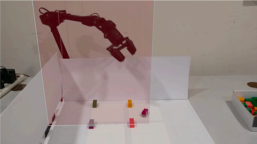
\includegraphics[width=0.9\linewidth]{figs/d-work-env.png}
    %         \caption{}
    %         \label{fig:sfig4}
    %     \end{subfigure}
    %     \caption{AR displayed work envelope of robotic arm \cite{CHU2023313}}
    %     \label{fig:ar-envelope}
    % \end{figure}
    

%     %notas para adicionar sobre o artigo - acima - 
%     The experiment aims to verify and
%     cross-compare the effectiveness of visual and haptic cues in various forms that convey the robot intent to human.
%     Analysis of the work performance and gazing behavior of participants shows that both cues can reduce their
%     visual attention on the moving robot during the collaboration. 
%     [10] emphasized the importance of human information
%     communication on assuring safety in HRC. They considered AR as an
%     ideal interface that enables the human and robot to ground their
%     communication and intentions by sharing an ego-centric view. AR also
%     allows for an exocentric view of the collaborative workspace that provides spatial awareness. This study suggested that a human-robot
%     collaborative system based on multimodal interactions would be more
%     effective and natural than unimodal.
%     Since  AR headsets still have a very limited field of view compared to the human vision. Visual guidance for localizing out-of-view objects in the limited display space often causes visual conflicts such as cluttering or occlusion of information [11]
%     Other works [12] proposed a visualization interface in AR HMD that superimposed the intended robot motion onto the user’s
%     view of real environment verifying that  the user determined where the robot was going to move using the interface more
%     quickly and accurately than 2D display or no assisted visualization.

%     the article itself outlines that providing AR user interfaces with either visual, haptic or multi-modal cues for HRC are benefitial.
%         Visual-based AR (cues) help overcome limitations arising from complex environments by superimposing visuals in an HMD without compromising robot mobility. this system also revealed to reduce the idle robot time as well as the task completion time when compared to the baseline without the user interface or the space sharing. However, user experience assessment showed that the HoloLens setup was not yet technically mature on the shop floor, particularly the limited field of view.
%         Visual feedback on a screen displayed the swept volume generated by the planned robot trajectory. Experimental data indicated that the human
%         workers felt more comfortable and had a better understanding of the robot motion and goals using multi-modal feedback. 
%         Haptic cues - It is sometimes advantageous in industrial environments over visual and auditory modalities, which could be overloaded or blocked on site. Vibrotactile devices have been applied to control industrial robot and to inform users of approaching singularities and joint limits in a factory [22]
%         Visual and acustic - aimed to reduce human's anxiety related to the unpredictability of the robot motion in a shared workspace. Acoustic feedback was used to alert the human when the robot had detected a possible collision and changed the planned motion.

%         % \ac{ROS} was useful, said by this article, this reinforces that the model i developed goes in line to what the literature supports
%         Implementing the system using the Robot Operating System also allowed modularity and extendibility for such a multi-device and multi-user approach.

%         % see conclusion - were the visual and haptic cues that communicated the robot motion useful in a collaborative assembly for the user?

%         % experiment:
%         During the assembly, a human operator picks, fetches, and stacks LEGO blocks onto specific work areas determined by the block color, while a desktop robot transports extra blocks to the areas over a wall.

%         In addition, both visual and tactile cues are presented in two forms that convey the robot motion with different degrees of information in AR.

%         % display 
%         As shown in figure \ref{f:area-1}, the operator was collaborating with a robot arm in a 25 cm × 25 cm work space in the middle of the table. The space was divided into four areas and each held LOGO blocks of a different color (see Fig. 2). The robot arm was mounted outside of the work space separated by a wall.

%         \begin{figure}[!htpb]
%             \centering
%             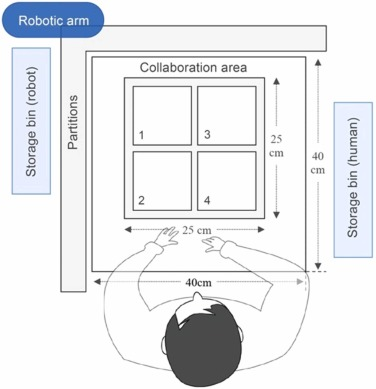
\includegraphics[width=0.4\linewidth]{figs/area-1.jpg}
%             \caption{Collaborative work space in the experiment, \cite{CHU2023313}}
%             \label{f:area-1}
%         \end{figure}

%         The space was divided into four areas and each held LOGO blocks of a different color (see figure \ref{f:robot-area-1}). The robot arm was mounted outside of the work space separated by a wall.

%         \begin{figure}[!htpb]
%             \centering
%             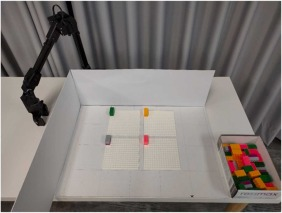
\includegraphics[width=0.4\linewidth]{figs/robot-area-1.jpg}
%             \caption{Actual work environment in the experiment, \cite{CHU2023313}}
%             \label{f:robot-area-1}
%         \end{figure}

%         The human and the robot independently performed individual tasks without a physical contact during the experiment. The operator picked up a block randomly from a storage bin on the right; then assembled the block into the area corresponding to its color. The storage bin contained 12 blocks of each different color. In contrast, the robot picked up a block at random times from the storage area on the left, which contained 4 blocks of each color. It then delivered the block to one of the four areas, also at random. The manual assembly of LEGO blocks must comply with the
%         following instructions. First, only one block was assembled at one time.
%         The operator could finish the assembly by using one or both hands.
%         Second, a block must be assembled to the area matching its color. The
%         block assembly started from the upper left of each area; then sequentially progressed from left to right and from up to bottom. Next, a block
%         could not be placed on top of existing blocks. The operator was asked to
%         complete the tasks as efficient as possible, while avoiding any collision
%         or physical contact with the robot.

% % visual and haptic user implemented interfaces
%         The visual interface was implemented in the HoloLens 2, which displayed the robot’s planned motion and the swept volume generated by the robot trajectory. The visual interface was designed to provide the operator with a clear understanding of the robot’s intended motion and goals. The haptic interface was implemented using the SenseGlove Nova™, which provided force feedback to the operator’s hand. The haptic interface was designed to alert the operator of the robot’s planned motion and to guide the operator’s hand to the correct assembly location. they can be seen in the figure \ref{fig:haptic-visual-cues}.

%         \begin{figure}[htp]
%             \centering
%             \begin{subfigure}{.5\textwidth}
%                 \centering
%                 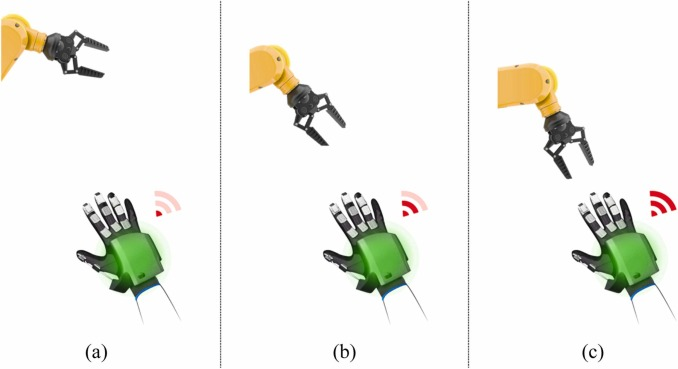
\includegraphics[width=0.9\linewidth]{figs/haptic-cues.jpg}
%                 \caption{Indicating the gripper’s destination using vibration on different human fingers.}
%                 \label{fig:sfig1}
%             \end{subfigure}%
%             \begin{subfigure}{.5\textwidth}
%                 \centering
%                 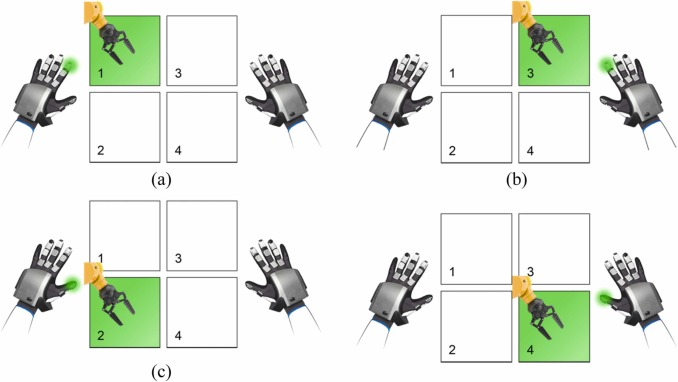
\includegraphics[width=0.9\linewidth]{figs/visual-cues.jpg}
%                 \caption{Indicating the proximity of gripper via change of vibration frequency.}
%                 \label{fig:sfig2}
%             \end{subfigure}
%             \label{fig:haptic-visual-cues}
%         \end{figure}
        

%         % AR interfaces - integration:
%         A WidowX 250 Robot Arm developed by Trossen Robotics was used
% in the experiment. This device is a 5-DOF desktop robotic arm with a
% 650-mm work range centered at the base. The robot
% control is realized by a computer through the Robot Operating System
% (\ac{ROS}) [42]. \ac{ROS} supports the motion planning framework MoveIt [43],
% which provides fundamental open-source functions for robot motion
% planning and manipulation. (this part is similar to the one of the project i am working with- robot with \ac{ROS} and also Moveit integrated - useful to mention)
% the manual tasks were performed while wearing a Microsoft HoloLens 2: The two visual interfaces were mainly implemented in HoloLens 2.
% We adopted SenseGlove Nova™, shown in figure \ref{f:HTC-gloves} to produce force feedback required
% by the haptic user interfaces. It is a programmable device commonly
% used in \ac{VR} applications to simulate tactile perception for
% high interactivity. To integrate the device with AR applications involves
% recognition of the user’s hand gesture and position in real environment.
% For this purpose, a HTC VIVE tracker was attached on each glove.

% \begin{figure}[!htpb]
%     \centering
%     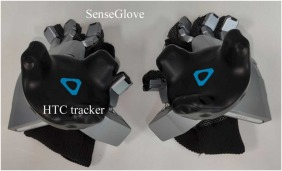
\includegraphics[width=0.6\linewidth]{figs/gloves.jpg}
%     \caption{Attaching HTC trackers on SenseGlove, \cite{CHU2023313}}
%     \label{f:HTC-gloves}
% \end{figure}

% Figure \ref{f:system-framework} shows the system framework proposed to integrate hardware
% devices with the UNITY engine residing on a desktop computer as an
% application server. The computer connected with the robot arm using a
% USB cable via Ubuntu v20.4 and executed motion control in \ac{ROS}. It
% communicated with the HoloLens 2 and SenseGlove using WiFi and
% Bluetooth, respectively.

% \begin{figure}[!htpb]
%     \centering
%     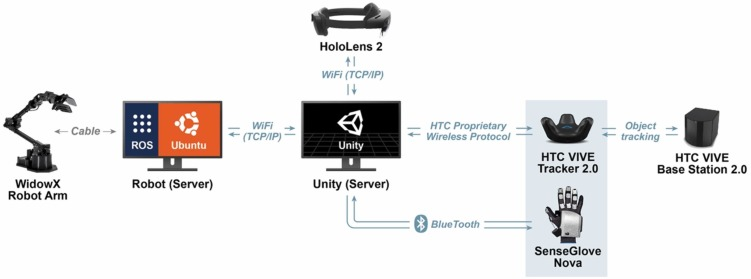
\includegraphics[width=0.6\linewidth]{figs/system-framework.jpg}
%     \caption{The system framework for integration of hardware devices in the experiment, \cite{CHU2023313}}
%     \label{f:system-framework}
% \end{figure}

% Section: Implementing AR and Digital Twins in Human-Robot Collaboration (HRC)

\paragraph{\textbf{Experiment Design: Collaborative LEGO Assembly Task}}
    The experimental setup involved a human operator collaborating with a desktop robotic arm in a 25 cm × 25 cm workspace. The operator's task was to pick, fetch, and stack LEGO blocks onto specific areas of the workspace, sorted by color, while the robot arm delivered extra blocks randomly into the workspace over a wall. It aimed to verify and cross-compare the effectiveness of visual and haptic cues in conveying the robot’s intent to the human operator. Figures \ref{f:area-1} and \ref{f:robot-area-1} depict the collaborative workspace and robot setup.

    \begin{figure}[!htpb]
        \centering
        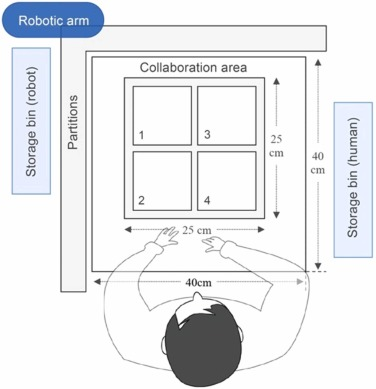
\includegraphics[width=0.4\linewidth]{figs/area-1.jpg}
        \caption{Collaborative work space in the experiment \cite{CHU2023313}}
        \label{f:area-1}
    \end{figure}

    \begin{figure}[!htpb]
        \centering
        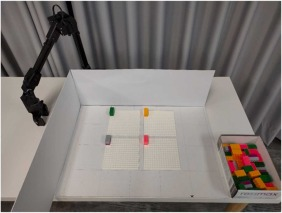
\includegraphics[width=0.4\linewidth]{figs/robot-area-1.jpg}
        \caption{Actual work environment in the experiment \cite{CHU2023313}}
        \label{f:robot-area-1}
    \end{figure}

    \paragraph{\textbf{System Framework}}
    UNITY engine running on a desktop computer allowed to communicat with the robot and the \ac{AR} devices. As shown in figure \ref{f:system-framework}, the system's architecture used USB connections and WiFi/Bluetooth for communication between the HoloLens, SenseGlove, and Robot. A HTC VIVE tracker was attached to the gloves to track the user's hand movements, providing haptic feedback in synchronization with the \ac{AR} visuals.

% remove this figure (done) - change the above text to reflect the removal of the figure
    % \begin{figure}[!htpb]
    %     \centering
    %     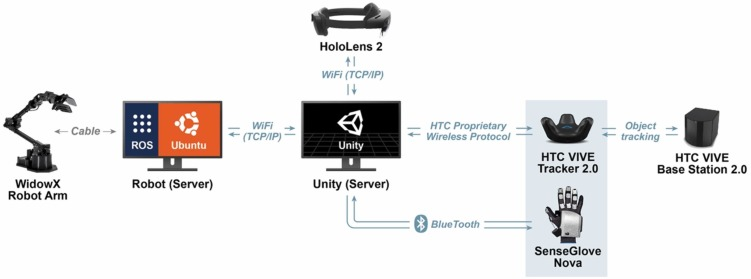
\includegraphics[width=0.75\linewidth]{figs/system-framework.jpg}
    %     \caption{The system framework for integration of hardware devices in the experiment \cite{CHU2023313}}
    %     \label{f:system-framework}
    % \end{figure}

    The framework allowed seamless interaction between the physical and virtual worlds, enabling real-time feedback for the operator, thus improving decision-making and task efficiency in the assembly process.



    % \paragraph{Conclusion}
    % The experiment with LEGO assembly and the integration of \ac{AR} and haptic feedback showed that visual and haptic \ac{AR} interfaces effectively communicate robot motion intent, improving interaction and collaboration. The system, using \ac{ROS} and MoveIt, provided a flexible and scalable platform for HRC in a shared workspace. The findings of this study align well with current literature, which emphasizes the importance of multimodal feedback in enhancing human-robot interaction in smart manufacturing.

%  parece-me que a parte de cima parece estar bem estruturada e revelar as vantagens do artigo explorado - ver as referencias que faltam e organizar melhor a estrutura e as figuras - remover depois o texto comentado que está acima de toda esta parte que escrevi agora - 24 set 01h56

    %verificar este artigo e mencionar coisas mais úteis, isto está mto breve
    % Additionally, Lotsaris et al.~\cite{LOTSARIS2021301} presented an \ac{AR} application that facilitates operator work in human-robot environments by 
    % enabling coexistence and improving communication. Their system displays safety fields around the robot using different colors to represent safe and 
    % dangerous regions, enhancing situational awareness and reducing the risk of accidents. However, a significant challenge remains in the complexity of
    % recognizing detailed information through haptic feedback, indicating a need for more sophisticated algorithms and sensors to capture and translate 
    % complex robot actions into intuitive \ac{AR} visualizations.
    


%%%%%%%%%%%%%%%%%%%%%%%%%%%%% 24 set - 17h - deixar ??? ver o que este artigo diz e se é relevante
    % \item \textbf{Virtual and Augmented Reality for Intuitive Robot Programming}
    
    % Programming robots using Virtual Reality (VR) and \ac{DT} introduces innovative methods that capture human movements, reducing the learning curve for 
    % non-experts and enabling intuitive programming of complex tasks. Bolano et al.~\cite{Bolano2020} demonstrated that bilateral communication between 
    % the VR environment and the robot’s hardware allows changes to be made in both the virtual and physical systems. This full immersive experience 
    % enables users to interact directly with the robot's end effector through holographic interfaces, facilitating the selection and application of 
    % desired operations seamlessly.
    
    % Similarly, Burghardt et al.~\cite{burghardt2020programming} explored programming DTs using VR, where the robot reproduces human movements within a virtual 
    % environment. This approach ensures that the robot can accurately mimic complex human actions, which is particularly beneficial in tasks that are 
    % challenging to automate traditionally. The integration of Unity and \ac{ROS} platforms further enhances the functionality by 
    % providing robust communication and real-time data processing capabilities.
    
    % In the context of mobile platforms, Lotsaris et al.~\cite{LOTSARIS2021301} highlighted the challenges of achieving friendly interaction in shared 
    % working environments due to the absence of effective communication between operators and robots. Their AR application addresses this by displaying 
    % safety fields and facilitating better communication, thereby improving the overall interaction experience.
    
    % \begin{figure}[h]
    %     \centering
    %     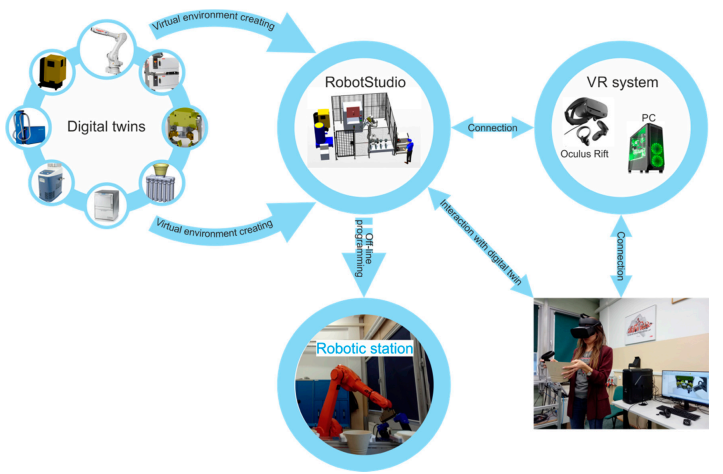
\includegraphics[width=0.9\linewidth]{figs/vr-oculos-dt.png}
    %     \caption{Schematic diagram of the building and programming of a robotic station alongside VR technologies \cite{burghardt2020programming}}
    %     \label{fig:vr-oculos-dt}
    % \end{figure}
    
    % Despite these advancements, challenges such as the need for high precision in replicating human movements and the complexity of \ac{VR} tracking 
    % technology persist. Improvements in algorithms, particularly those utilizing Machine Learning (\ac{ML}) techniques, are essential to ensure that 
    % robotic movements closely mimic human operators' actions \cite{Burghardt2020}.
    
